\section{Quest Package}
%TODO referenz folgt Quest Package erklärung
Hier kann man zwischen den vorhanden Quest Packages wählen. Wobei rechts die Beschreibung des jeweiligen Packages, falls diese vorhanden ist, angezeigt wird. Mithilfe eines Klicks auf den Pfeil kann das gewünschte Package ausgewählt werden.

\begin{figure}[h] 
  \centering
     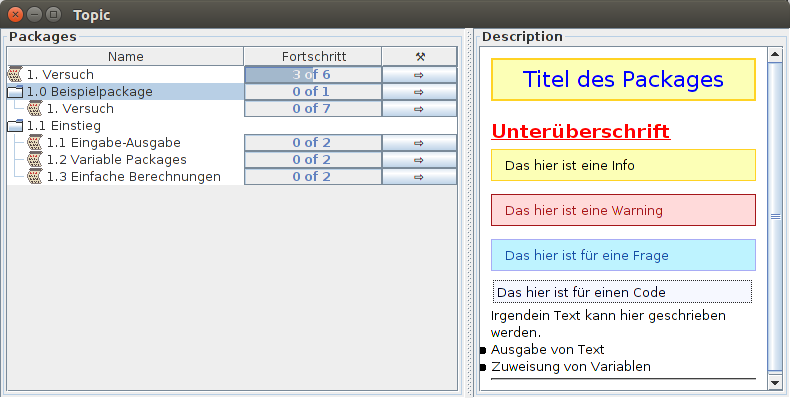
\includegraphics[width=1\textwidth]{./media/images/gui/package-auswahl.png}
  \caption{Auswahl des Packages}
  \label{fig:Package_Auswahl}
\end{figure}

Weiters wird auch der Fortschritt des Packages angezeigt. Daraus ist ersichtlich, wie viele Quests man in diesem Packet bereits fertiggestellt wurden.

Bei einem Quest Package wurde ein JTree\footnote{\url{http://www.hameister.org/JavaSwingTreeTable.html}}  zur Realisierung verwendet. Dieses befindet sich wiederum in einer JScrollpane. Somit ist die Anzahl der Elemente in der JTable\footnote{\url{https://docs.oracle.com/javase/tutorial/uiswing/components/scrollpane.html}}  , und somit eines Packages, nicht begrenzt.
